\newprob{1715500568}
{
下圖顯示一位摩托車騎手使用一個 \dg{20}的斜坡來跳過一條寬度為 10 m 的河流(摩托車和騎士可以被視為點粒子)。取 $g=9.81$。
{\par\centering
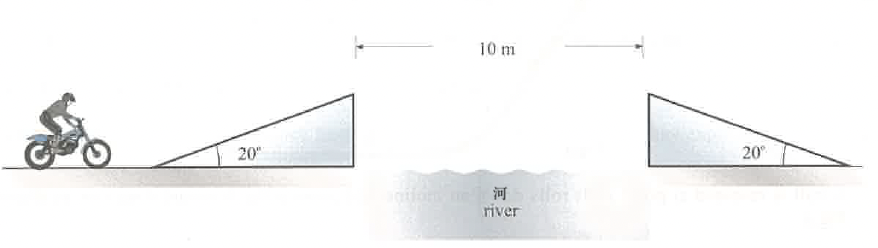
\includegraphics[width=.7\textwidth]{assets/607732e8.png}
\par}
\begin{parts}
    \part 計算騎手離開第一個斜坡的頂端的最小速度,使得他能安全地跨越到同等高度的第二個斜坡。\par\zzh{2}
    \part 使用(a)中的速度,計算摩托車達到斜坡上方的最大高度。\zzh{2}
\end{parts}
\dlines{1}
}{
\sol
\begin{enumerate}
    \item 水平方向 : $(u\cos 20^\circ)t=10$ \par
          $t=\dfrac{10}{u\cos 20^\circ}$\giveM\par
          垂直方向 : $0=(u\sin 20^\circ)t-\frac{1}{2}(9.81)t^2$\par
          $\dfrac{2u\sin 20^\circ}{9.81}=\dfrac{10}{u\cos 20^\circ}$\par
          $u=12.3538=\qty{12.4}{m.s^{-1}}$ \giveA
    \item $0^2-12.3538^2\sin^2 20^\circ=2(-9.81)H$\giveM\par
          $H=0.90993=\qty{0.910}{m}$\giveA
\end{enumerate}
}

\newprob{1715500724}
{
    在圖中,球員P以 \vel{28} 的速度以 \dg{30} 的角度將棒球擊出,初始高度比地面高 \qty{1}{m}。


    \begin{parts}
        \part
        初速度的垂直分量是多少?\zzh{1}
        \part 球需要多久才能返回到初始高度?\zzh{2}
        \part 球在返回到地面上方的初始高度前,水平前進了多遠的距離?\zzh{2}
        \part
        \topalign{\par\centering
            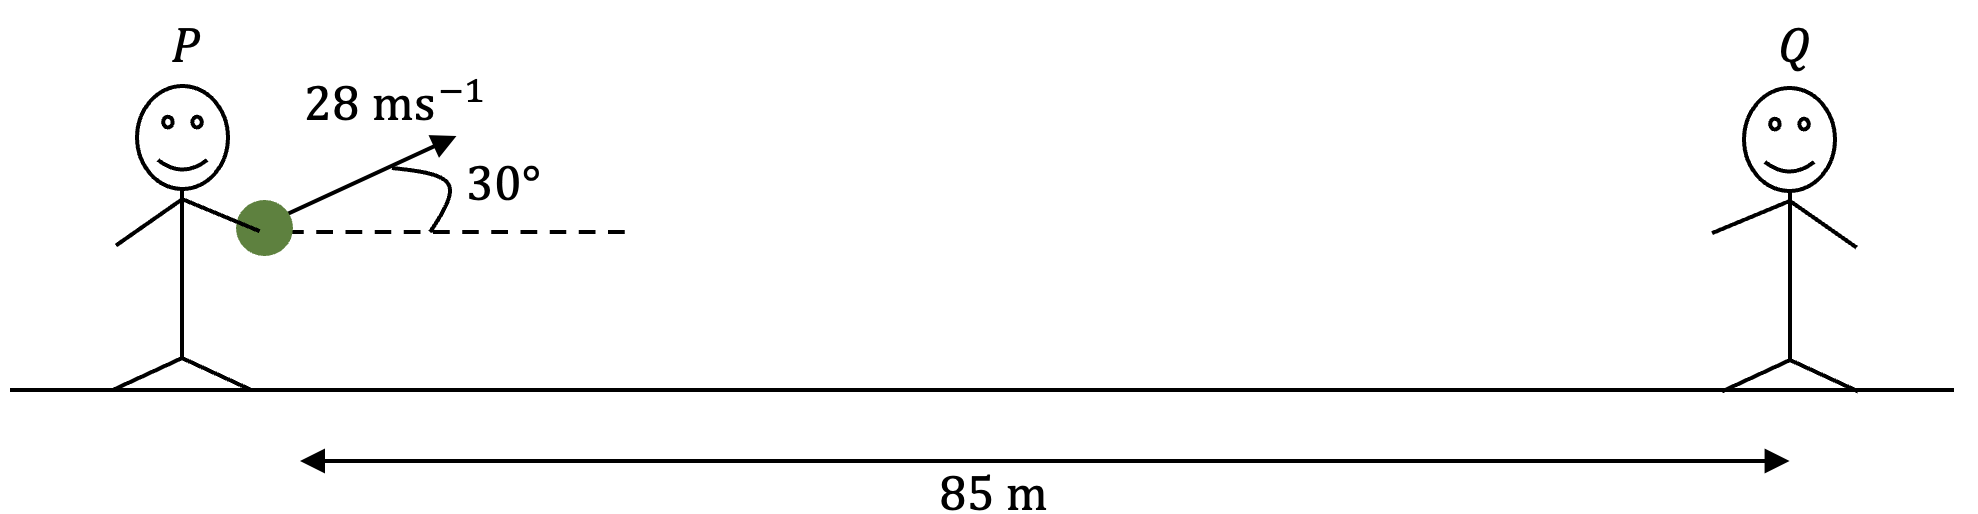
\includegraphics[width=.8\textwidth]{assets/11240120.png}
            \par}\par
        球直接朝著靜止的球員 Q 擊出,Q距離P有 \qty{85}{m},並在球被擊出的瞬間開始以恆定加速度向球跑去。如果他要在球距離地面 \qty{1}{m}的高度接住球,他的加速度量值是多少?\zzh{3}
    \end{parts}
    \dlines{1}\clearpage\dlines{1}
}{
    \begin{enumerate}
        \item $28\sin 30^\circ=\qty{14}{m.s^{-1}}$\giveA
        \item $0=(28\sin 30^\circ)t-\frac{1}{2}(9.81)t^2$\giveM\par
              $t=\dfrac{2(28\sin 30^\circ)}{9.81}=2.85423=\qty{2.85}{s}$\giveA
        \item $(2.85423)(28\cos 30^\circ)=69.2114=\qty{69.2}{m}$\giveMA
        \item $85-69.2114=\dfrac{1}{2}a(2.85423)^2$ \giveM \par
              $a=\qty{3.88}{m.s^{-2}}$\giveA
    \end{enumerate}
}

\newprob{1715500849}
{
一架飛機剛好在砲台的正上方時,砲台就開火了。假設飛機以水平速度 $u$ 前進,而砲彈的速度為 $v = 2u$。
{\par\centering
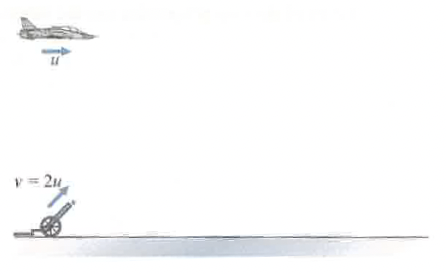
\includegraphics[width=.4\textwidth]{assets/565f9fec.png}
\par}
\begin{parts}
    \part
    要擊中飛機,投射的角度應該是多少?\zzh{2}

    \part
    計算飛機避免被砲彈擊中時,飛機距離地面的最小高度,以 $u$ 和 $g$ 表示。忽略空氣阻力。\zzh{3}

\end{parts}
\dlines{1}
}{
\begin{enumerate}
    \item
          $2u\cos\theta=u$\giveM\par
          $\cos\theta=\dfrac{1}{2}$\par
          $\theta=60^\circ$\par
          投射角$=60^\circ$\giveA
    \item $0-u^2\sin^2 60^\circ=2(-g)(H)$\giveM\par
          $H=\dfrac{3u^2}{8g}$\par
          $\therefore$ 最小高度 $=\dfrac{3u^2}{8g}$\giveA
\end{enumerate}

}

\newprob{1715501281}
{
一人把南瓜斜向上拋向 5 m 外的高塔,南瓜曲 墜,擊中塔身離地 18 m 的位置。所經軌跡的最 高點離地 20 m。
{\par\centering
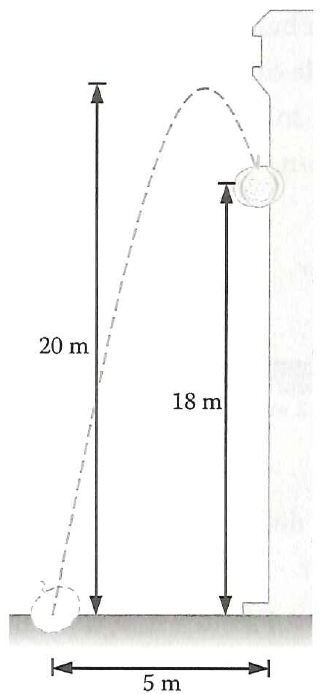
\includegraphics[width=0.2\linewidth]{assets/dwdqw.png}\par}
\begin{parts}
    \part 求南瓜的垂直初速率。\zzh{2}
    \part 求南瓜的飛行時間。\zzh{3}
    \part 由此或其他方法,求南瓜初速度的量值和 方向。\zzh{2}

\end{parts}
\dlines{1}\clearpage\dlines{1}
}{\par{\par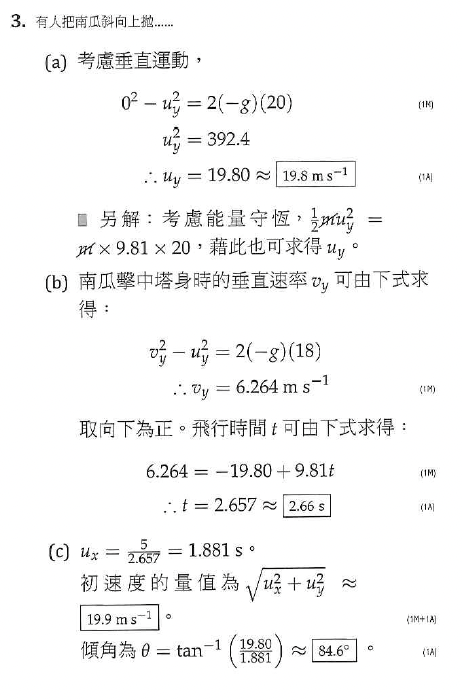
\includegraphics[width=0.75\linewidth]{assets/wqq2ge.png}}}